\documentclass{article}

\usepackage[a4paper, left=3cm,right=2cm,top=2.5cm,bottom=2.5cm]{geometry}
\usepackage{graphicx}
\usepackage{amsthm}
\usepackage[table]{xcolor}
\usepackage{listings}
\usepackage{tikz}

\usepackage{hyperref}
\hypersetup{
    colorlinks=true,
    linkcolor=blue,
    filecolor=magenta,      
    urlcolor=cyan,
}

\newtheorem{stelling}{Stelling}

\author{Lorenzo De Bie}
\title{Gegevensstructuren en Algoritmen}
\date{June 19, 2020}
\begin{document}

\maketitle

\tableofcontents

\newpage

\section{Inleiding\label{inleiding}}
\subsection{Analyse van algoritmen}
Uitvoeringstijd staat centraal. Vergelijken van algoritmes zonder implementatie en uitvoering.
Performatie afhankelijk van veel verschillende factoren:
\begin{itshape}
	\begin{itemize}
		\item programmeertaal
		\item programmeur = dummy of niet
		\item compiler
		\item processorarchitectuur
	\end{itemize}
\end{itshape}
Niet mogelijk om met al deze factoren rekening te houden \&\& ze bepalen dan ook enkel de uitvoeringstijd voor één enkele computer. Wel rekening houden met:
\begin{itemize}
 	\item Aantal verwerkte gegevens $n$
 	\item Oorspronkelijke volgorde
 	\item Statistische verdeling
\end{itemize}
Algoritme opdelen in aantal \textit{primitieve operaties}. Drie belangrijke situaties:
\begin{itemize}
	\item Best-case Running Time: $\Omega$-notatie\newline
	Ondergrens voor uitvoertijd:
	\item Worst-case Running Time: $O$-notatie\newline
	Bovengrens voor uitvoertijd
	\item Average-case Running Time: $\Theta$-notatie\newline
	Boven- en ondergrens voor uitvoertijd
\end{itemize}
Beschrijven stijging uitvoeringstijd ifv $n$
\begin{figure}[h]
	\centering
	\includegraphics[width=\textwidth]{Growth_of_functions}
	\caption{Voorbeelden van notaties}
	\label{fig:figure1}
\end{figure}

\subsection{Asymptotische Benadering van Functies\label{asymp_ben}}
Eigenschappen $O$-notatie:
\begin{itemize}
	\item $O(f(n)) + O(g(n)) = O(max(f(n),g(n)))$
	\item $O(c \cdot f(n)) = O(f(n))$
	\item $f(n) = O(g(n))$ en $g(n) = O(h(n)) \Rightarrow f(n) = O(h(n))$
	\item $f(n) = O(f(n))$
\end{itemize}

Per probleem asymptotische efficiëntie van efficiëntste oplossing bepalen niet altijd mogelijk (P vs NP-problemen). Sorteren wel al gekend:

\begin{stelling}
Keuze tussen $f(n)$ elementen is $\Theta(\lg f(n))$ en door Stirling wordt sorteren dus $\Theta(n\lg(n))$
\end{stelling}

Dit stuk van de cursus is echt brak so we move on

\newpage

\section{Rangschikken\label{rangschikken}}
\subsection{Insertion Sort} % (fold)
\label{sub:insertion_sort}
\subsubsection{Doel} % (fold)
\label{sub:ins_sort_doel}
Sorteren van elementen.
% subsubsection doel (end)

\subsubsection{Basisprincipes} % (fold)
\label{sub:ins_sort_basisprincipes}
Starten met een gesorteerde tabel van één element (is al gesorteerd). Iedere keer volgende element bijnemen en dan \textit{tussenvoegen} op de juiste plaats door grotere elementen één voor één een plaats op te schuiven (\textit{lineair zoeken}, beginnend bij kleinste of grootste element). Als het nieuwe element op de juiste plaats staat hebben we een gesorteerde tabel met één element meer. Dit proces wordt herhaald tot de tabel gesorteerd is. Insertion sort sorteert \textit{ter plaatse} want het gebruikt enkel de oorspronkelijke tabel en het aantal hulpvariabelen hangt niet af van $n$. Stabiel sorteren is mogelijk als er strikt vergeleken wordt.
% subsubsection basisprincipes (end)

\subsubsection{Voorbeeld} % (fold)
\label{sub:ins_sort_voorbeeld}
Rij om te sorteren: Eerste cijfer is al gesorteerd want rij van één cijfer is altijd oké.
Rood = getal dat nu tussengevoegd wordt.
\begin{center}
\begin{tabular}{ |c|c|c|c|c| }
\hline
\cellcolor{gray}2 & \cellcolor{red}3 & 1 & 5 & 4 \\
\hline
\end{tabular}
\end{center}
Geen opschuivingen nodig.
\begin{center}
\begin{tabular}{ |c|c|c|c|c| }
\hline
\cellcolor{gray}2 & \cellcolor{gray}3 & \cellcolor{red}1 & 5 & 4 \\
\hline
\end{tabular}
\end{center}
Hier moet het cijfer meerdere plaatsen opschuiven: dit gaat één plaats per keer:
\begin{center}
\begin{tabular}{ |c|c|c|c|c| }
\hline
\cellcolor{gray}2 & \cellcolor{red}1 & \cellcolor{gray}3 & 5 & 4 \\
\hline
\end{tabular}
\end{center}
Dit doen we zo verder tot de volledige rij gesorteerd is:
\begin{center}
\begin{tabular}{ |c|c|c|c|c| }
\hline
\cellcolor{gray}1 & \cellcolor{gray}2 & \cellcolor{gray}3 & \cellcolor{red}5 & 4 \\
\hline
\end{tabular}
\end{center}
\begin{center}
\begin{tabular}{ |c|c|c|c|c| }
\hline
\cellcolor{gray}1 & \cellcolor{gray}2 & \cellcolor{gray}3 & \cellcolor{gray}5 & \cellcolor{red}4 \\
\hline
\end{tabular}
\end{center}
\begin{center}
\begin{tabular}{ |c|c|c|c|c| }
\hline
\cellcolor{gray}1 & \cellcolor{gray}2 & \cellcolor{gray}3 & \cellcolor{gray}4 & \cellcolor{gray}5 \\
\hline
\end{tabular}
\end{center}
Het is duidelijk dat iedere keer de grotere elementen één plaats opschuiven, en het nieuwe element \textit{tussengevoegd} wordt op de juiste plaats.
% subsection voorbeeld (end)

\subsubsection{Complexiteit} % (fold)
\label{sub:ins_sort_complexiteit}
\begin{itemize}
	\item Best-case: $\Theta(n)$
	Tabel is al gesorteerd: er zijn dus geen inversies. \textbf{Ook voor bijna gesorteerde tabellen.}
	\item Average-case: $\Theta(n^2)$
	Iedere permutatie is even waarschijnlijk: half zoveel inversies als worst-case.
	\item Worst-case: $\Theta(n^2)$
	Tabel staat in omgekeerde volgorde: elk paar elementen is een inversie.
\end{itemize}
% subsection complexiteit (end)

\subsubsection{Waarom beter?} % (fold)
\label{sub:ins_sort_waarom_beter}
Grote voordeel van insertion sort is dat het voor \textit{bijna gesorteerde} tabellen ook $\Theta(n)$ is. Het werkt dus goed om elemeten toe te voegen aan een al gesorteerde tabel. Het wordt ook gebruikt in de slotfase van enkele andere (over het algemeen efficiëntere) algoritmen.
% subsection waarom_beter_ (end)

\subsubsection{Mogelijke optimalisaties?} % (fold)
\label{sub:ins_sortmogelijke_optimalisaties}
\begin{itemize}
	\item Binair zoeken gebruiken om juiste plaats te vinden voor \textit{tussenvoegen}. \textbf{Wel opletten dat algoritme stabiel blijft!}
	\item Grootste probleem is dat er \textbf{maar één inversie per verschuiving} opgelost wordt. Meerdere inversies oplossen per verschuiving zal de performantie verbeteren $\Rightarrow$ \textit{Shell sort}
	\item Gebruik van \textit{swap-operatie} ipv opschuiven kan beter zijn voor grotere klassen.
	\item Voor begin binnenste lus checken of nieuw getal kleiner is dan kleinste (of groter dan grootste) $\Rightarrow$ direct voorraan (of achteraan) plaatsen
\end{itemize}
% subsection mogelijke_optimalisaties_ (end)

\subsubsection{Analyse/Bewijs complexiteit} % (fold)
\label{sub:ins_sort_analyse_bewijs_complexiteit}
De complexiteit van insertion sort hangt af van het aantal inversies in de tabel. Er zijn twee \textit{genneste} lussen: één die over alle ementen loopt ($n-1$ keer uitgevoerd, en dus $\Theta(n)$), en de binnenste herhaling die sleutelvergelijkingen en schuifoperaties uitvoert. Iedere schuifoperatie verwijdert één inversie. Voor iedere schuifoperatie is er één sleutelvergelijking, en mogelijks nog één extra sleutelvergelijking per element.
Het aantal sleutelvergelijkingen is dus $O(\#inversies + n)$
\begin{itemize}
	\item Worst-case: elk paar elementen vormen een inversie (tabel in omgekeerde volgorde). $n(n-1)/2$ paren van elementen en dus evenveel schuifoperaties. Het aantal sleutelvergelijkingen is dus $O(n(n-1)/2 + n)$. De totale uitvoertijd is dus $\Theta(n^2)$ aangezien alle andere operaties $\Theta(n)$ zijn.
	\item Average-case: alle permutaties van tabel even waarschijnlijk $\Rightarrow$ helft zoveel inversies $n(n-1)/4$. Gemiddeld $\Theta(n^2)$ schuifoperaties en $O(n^2 + n)$ sleutelvergelijkingen. Complexiteit blijft dezelfde: $\Theta(n^2)$.
	\item Best-case: geen inversies, geen kwadratische term $\Rightarrow \Theta(n)$. \textbf{Als het aantal inversies $O(n)$ blijft zal insertion sort ook $\Theta(n)$ blijven.} Bijna gesorteerde tabellen kunnen dus ook $\Theta(n)$ gesorteerd worden.
\end{itemize}
% subsection analyse_bewijs_complexiteit (end)
% subsection insertion_sort (end)


\subsection{Shell sort} % (fold)
\label{sub:shell_sort}
\subsubsection{Doel} % (fold)
\label{sub:shell_sort_doel}
Zelfde als \hyperref[sub:insertion_sort]{Insertion Sort}: sorteren van elementen.
% subsection doel (end)

\subsubsection{Basisprincipes} % (fold)
\label{sub:shell_sort_basisprincipes}
Shell sort is een uitbreiding op \hyperref[sub:insertion_sort]{Insertion Sort}. \hyperref[sub:insertion_sort]{Insertion Sort} is traag omdat het bij elke stap een element maar één plaats opschuift en dus maar één inversie oplost. Shell sort probeert elementen te wisselen die verder van elkaar liggen en dus meerdere inversies in één keer op te lossen. Om dit te doen wordt een tabel \textit{`k-gerankshikt'} met steeds kleinere \textit{`k'} (kleinste \textit{`k'} $= 1$ om volledig gerangschikte tabel te garanderen). Dit algortime steunt dus op het principe dat de ordering van hogere \textit{`k'} blijft bij het opnieuw rangschikken met kleinere \textit{`k'}. Het bewijs hiervoor is echt te brak uitgelegd dus \textit{good luck}. Shell sort rangschikt \textit{ter plaatse}, maar is niet \textit{stabiel}. Bij het sorteren van de deelreeksen kan de volgorde van gelijke sleutels wisselen.
% subsection basisprincipes (end)

\subsubsection{Voorbeeld} % (fold)
\label{sub:shell_sort_voorbeeld}
\begin{center}
\begin{tabular}{ |c|c|c|c|c|c|c|c|c| }
\hline
\cellcolor{gray!25}54 & \cellcolor{gray!50}26 & \cellcolor{gray!75}93 & \cellcolor{gray!25}17 & \cellcolor{gray!50}77 & \cellcolor{gray!75}31 & \cellcolor{gray!25}44 & \cellcolor{gray!50}55 & \cellcolor{gray!75}20 \\
\hline
\end{tabular}
\end{center}
We kunnen de tabel eerst \textit{`k'-rangschikken} met \textit{`k'}$ = 3$. Om deze deeltabellen te rankshikken kan insertion sort gebruikt worden omdat de deeltabellen veel kleiner zijn. Naarmate de deeltabellen terug groter worden zijn ze wel meer gerankshikt, dus is insertion dan ook nog altijd een goede oplossing.\newline
\begin{center}
\begin{tabular}{ |c|c|c|c|c|c|c|c|c| }
\hline
\cellcolor{gray!25}17 & \cellcolor{gray!50}26 & \cellcolor{gray!75}20 & \cellcolor{gray!25}44 & \cellcolor{gray!50}55 & \cellcolor{gray!75}31 & \cellcolor{gray!25}54 & \cellcolor{gray!50}77 & \cellcolor{gray!75}93 \\
\hline
\end{tabular}
\end{center}
Nu kunnen we deze tabel \textit{`2'-rangschikken}.
\begin{center}
\begin{tabular}{ |c|c|c|c|c|c|c|c|c| }
\hline
\cellcolor{gray!25}17 & \cellcolor{gray!50}26 & \cellcolor{gray!25}20 & \cellcolor{gray!50}44 & \cellcolor{gray!25}55 & \cellcolor{gray!50}31 & \cellcolor{gray!25}54 & \cellcolor{gray!50}77 & \cellcolor{gray!25}93 \\
\hline
\end{tabular}
\end{center}
Wordt dus:
\begin{center}
\begin{tabular}{ |c|c|c|c|c|c|c|c|c| }
\hline
\cellcolor{gray!25}17 & \cellcolor{gray!50}26 & \cellcolor{gray!25}20 & \cellcolor{gray!50}31 & \cellcolor{gray!25}54 & \cellcolor{gray!50}44 & \cellcolor{gray!25}55 & \cellcolor{gray!50}77 & \cellcolor{gray!25}93 \\
\hline
\end{tabular}
\end{center}
Als laatste \textit{`1'-rangschikken} (wat dus gewoon neer komt op insertion sort) deze tabel. Omdat deze tabel al zo goed als gesorteerd is zal de performantie hier ook goed zijn (\hyperref[sub:ins_sort_complexiteit]{insertion sort is $\Theta(n)$ voor bijna gesorteerde tabellen.}) Resultaat:
\begin{center}
\begin{tabular}{ |c|c|c|c|c|c|c|c|c| }
\hline
17 & 20 & 26 & 31 & 44 & 54 & 55 & 77 & 93 \\
\hline
\end{tabular}
\end{center}
% subsection voorbeeld (end)

\subsubsection{Complexiteit} % (fold)
\label{sub:shell_sort_complexiteit}
De complexiteit van shell sort hangt af van de reeks \textit{`k'} waarden die gebruikt worden. Gewoonlijk neemt ben een waarde kleiner dan $n/2$ als beginwaarde voor \textit{`k'}. Er zijn veel verschillende reeksen voor \textit{`k'}-waarden bekend, maar optimale reeks nog niet bekend.
% subsection complexiteit (end)

\subsubsection{Waarom Beter?} % (fold)
\label{sub:shell_sort_waarom_beter}
\begin{itemize}
	\item Aanzienlijk sneller dan \hyperref[sub:insertion_sort]{insertion sort}, blijft ook zeer goed presteren voor grotere $n$.
	\item Eenvoudigere methode dan asymptotisch snellere algoritmen.
\end{itemize}

% subsection waarom_beter_ (end)

\subsubsection{Mogelijke Optimalisaties} % (fold)
\label{sub:shell_sort_mogelijke_optimalisaties}
Enkel de reeksen voor \textit{`k'-waarden} kan geoptimaliseerd worden.
% subsection mogelijke_optimalisaties (end)

\subsubsection{Analyse/Bewijs complexiteit} % (fold)
\label{sub:shell_sort_analyse_bewijs_complexiteit}
Niet gegeven aangezien afhankelijk van reeks \textit{`k'-waarden}.
% subsection analyse_bewijs_complexiteit (end)
% subsection shell_sort (end)

\subsection{Selection Sort} % (fold)
\label{sub:selection_sort}
\subsubsection{Doel} % (fold)
\label{sub:sel_sort_doel}
Sorteren van elementen.
% subsection doel (end)

\subsubsection{Basisprincipes} % (fold)
\label{sub:sel_sort_basisprincipes}
Grootste element uit de tabel zoeken, en wisselen met het laatste element. Uit de overgebleven elementen het grootste zoeken en wisselen met het voorlaatste. Zo verder gaan tot de volledige tabel gerangschikt is. Selection sort rangschikt ter plaatse maar is niet stabiel. De definitieve gerangschikte tabel wordt element per element geconstrueerd: na iedere iteratie staan de laatste $i$ elementen op de juiste plaats (in tegenstelling tot \hyperref[sub:insertion_sort]{insertion sort}, waar de defintieve plaats van ieder element maar gekend is op het einde).
% subsection basisprincipes (end)

\subsubsection{Voorbeeld} % (fold)
\label{sub:sel_sort_voorbeeld}
Het grootste element is iedere keer rood ingekleurd en wordt verwisseld met het laatste nog niet grijze element.
\begin{center}
\begin{tabular}{ |c|c|c|c|c| }
\hline
2 & 3 & 1 & \cellcolor{red}5 & 4 \\
\hline
\end{tabular}

\begin{tabular}{ |c|c|c|c|c| }
\hline
2 & 3 & 1 & \cellcolor{red}4 & \cellcolor{gray}5 \\
\hline
\end{tabular}

\begin{tabular}{ |c|c|c|c|c| }
\hline
2 & \cellcolor{red}3 & 1 & \cellcolor{gray}4 & \cellcolor{gray}5 \\
\hline
\end{tabular}

\begin{tabular}{ |c|c|c|c|c| }
\hline
\cellcolor{red}2 & 1 & \cellcolor{gray}3 & \cellcolor{gray}4 & \cellcolor{gray}5 \\
\hline
\end{tabular}

\begin{tabular}{ |c|c|c|c|c| }
\hline
\cellcolor{red}1 & \cellcolor{gray}2 & \cellcolor{gray}3 & \cellcolor{gray}4 & \cellcolor{gray}5 \\
\hline
\end{tabular}

\begin{tabular}{ |c|c|c|c|c| }
\hline
\cellcolor{gray}1 & \cellcolor{gray}2 & \cellcolor{gray}3 & \cellcolor{gray}4 & \cellcolor{gray}5 \\
\hline
\end{tabular}
\end{center}
% subsection voorbeeld (end)

\subsubsection{Complexiteit} % (fold)
\label{sub:sel_sort_complexiteit}
Selection sort is $\Theta(n^2)$.
% subsection complexiteit (end)

\subsubsection{Waarom Beter?} % (fold)
\label{sub:sel_sort_waarom_beter}
Deze methode wordt nauwelijks gebruikt, omdat ze eigenlijk gewoon slecht is. Als de selectieprocedure beter wordt kan het wel een goede methode opleveren.
% subsection waarom_beter_ (end)

\subsubsection{Mogelijke Optimalisaties} % (fold)
\label{sub:sel_sort_mogelijke_optimalisaties}
Betere selectieprocedure. \hyperref[sub:heap_sort]{Heap Sort} is hier een voorbeeld van.
% subsection mogelijke_optimalisaties (end)

\subsubsection{Analyse/Bewijs complexiteit} % (fold)
\label{sub:sel_sort_analyse_bewijs_complexiteit}
Het aantal sleutelvergelijkingen is onafhankelijk van de volgorde van de elementen. Het aantal verwisselingen is hoogstens $n-1$ en dus $O(n)$. Het aantal keer dat het maximum aangepast wordt hangt samen met het aantal sleutelvergelijkingen 
\begin{center}
$(n-1) + (n-2) + ... + 2 + 1 = n(n-1)/2$
\end{center}
Aantal keer dat het maximum aangpast wordt is dus $O(n^2)$. Dit zorgt er voor dat selection sort een $\Theta(n^2)$ algoritme is.
% subsection analyse_bewijs_complexiteit (end)
% subsection selection_sort (end)

\subsection{Heap Sort} % (fold)
\label{sub:heap_sort}
\subsubsection{Doel} % (fold)
\label{sub:heap_sort_doel}
Sorteren van elementen
% subsection doel (end)

\subsubsection{Basisprincipes} % (fold)
\label{sub:heap_sort_basisprincipes}
Eerst wordt de tabel getransorfmeerd tot \textit{heap}. Nu kan het maximum van de tabel veel efficiënter gevonden worden (het is namelijk altijd het eerste element in de tabel). Door nu telkens de wortel van de heap te wisselent met het laatste element van de heap wordt de gerangschikte rij geconstrueerd. Na iedere wissel moet de \textit{heapvoorwaarde} wel hersteld worden. Voor meer informatie over de operaties op \textit{heaps} en hoe ze opgesteld worden verwijs ik naar het deel \hyperref[sub:heaps]{Heaps} bij \hyperref[gegI]{Gegevensstructuren I}. Heap sort rangschikt ter plaatse maar is niet stabiel. De volgorde van gelijke elementen kan veranderen bij de heapconstructie en herstellen \textit{heapvoorwaarde}.
% subsection basisprincipes (end)

\subsubsection{Voorbeeld} % (fold)
\label{sub:heap_sort_voorbeeld}
\begin{center}
\begin{tabular}{ |c|c|c|c|c|c|c|c|c|c| }
\hline
4 & 1 & 3 & 2 & 16 & 9 & 10 & 14 & 8 & 7 \\
\hline
\end{tabular}
\end{center}
Deze tabel wordt eerst omgezet naar een heap door samenvoegen van deelheaps. We beginnen met volgende boom:
\begin{center}
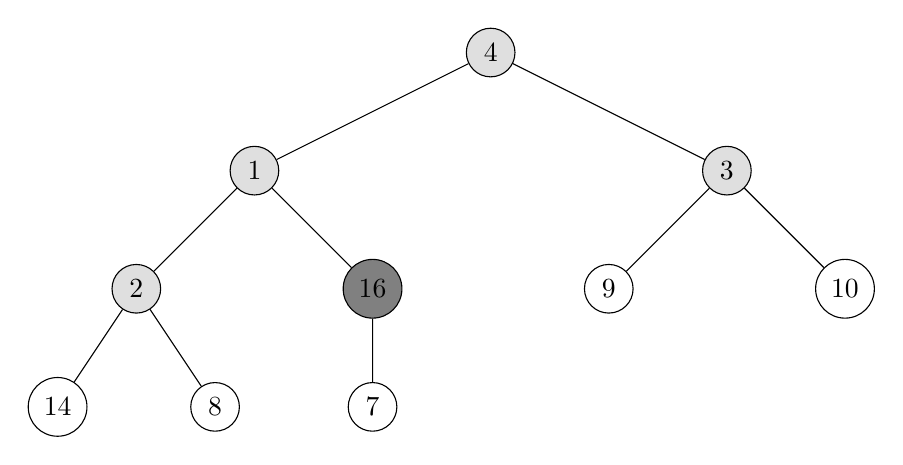
\begin{tikzpicture}[level/.style={sibling distance=60mm/#1}]
\node [circle,draw, fill=gray!25] (z){4}
	child {node [circle, draw, fill=gray!25] (a) {1}
		child {node [circle, draw, fill=gray!25] (c) {2}
			child {node [circle, draw] (g) {14}}
			child {node [circle, draw] (h) {8}}
		}
		child {node [circle, draw, fill=gray] (d) {16}
			child {node [circle, draw] (i) {7}}
		}
	}
	child {node [circle, draw, fill=gray!25] (b) {3}
		child {node [circle, draw] (e) {9}}
		child {node [circle, draw] (f) {10}}
	}
;
\end{tikzpicture}
\end{center}
De nog grijs ingekleurde cellen moeten eventueel nog zakken om aan de heapvoorwaarde te voldoen. We beginnen met de knoop met waarde 16. Deze heeft geen kinderen met een grotere waarde. Volgende knoop is deze met waarde 2, deze heeft een kind met grotere waarde, we wisselen altijd met het kind met de grootste waarde.
\begin{center}
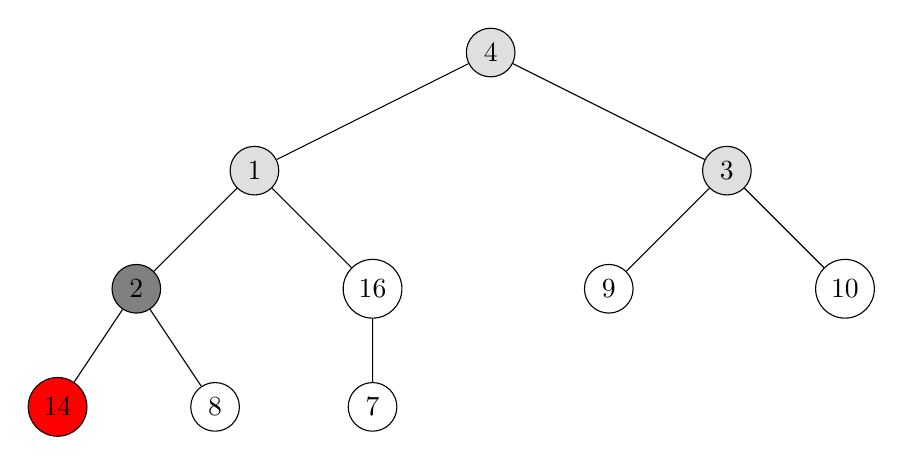
\begin{tikzpicture}[level/.style={sibling distance=60mm/#1}]
\node [circle,draw, fill=gray!25] (z){4}
	child {node [circle, draw, fill=gray!25] (a) {1}
		child {node [circle, draw, fill=gray] (c) {2}
			child {node [circle, draw, fill=red] (g) {14}}
			child {node [circle, draw] (h) {8}}
		}
		child {node [circle, draw] (d) {16}
			child {node [circle, draw] (i) {7}}
		}
	}
	child {node [circle, draw, fill=gray!25] (b) {3}
		child {node [circle, draw] (e) {9}}
		child {node [circle, draw] (f) {10}}
	}
;
\end{tikzpicture}
\end{center}
De volgende knoop is deze met waarde 3. Deze wordt gewisseld met deze met waarde 10.
\begin{center}
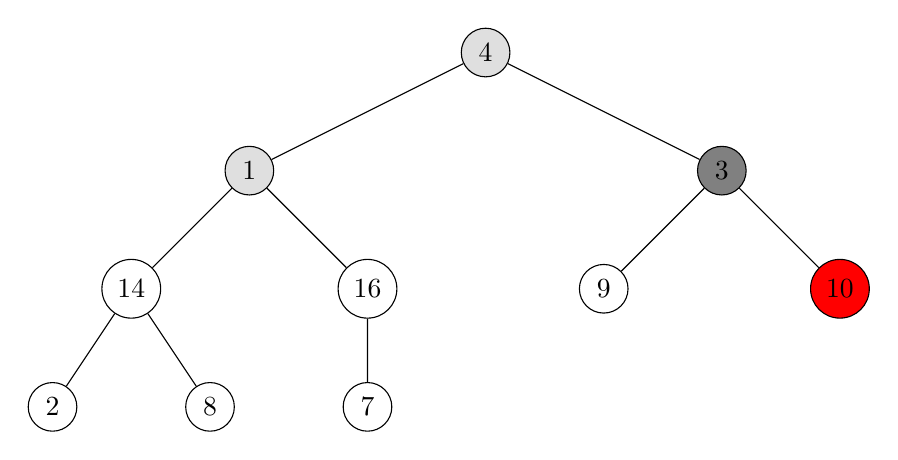
\begin{tikzpicture}[level/.style={sibling distance=60mm/#1}]
\node [circle,draw, fill=gray!25] (z){4}
	child {node [circle, draw, fill=gray!25] (a) {1}
		child {node [circle, draw] (c) {14}
			child {node [circle, draw] (g) {2}}
			child {node [circle, draw] (h) {8}}
		}
		child {node [circle, draw] (d) {16}
			child {node [circle, draw] (i) {7}}
		}
	}
	child {node [circle, draw, fill=gray] (b) {3}
		child {node [circle, draw] (e) {9}}
		child {node [circle, draw, fill=red] (f) {10}}
	}
;
\end{tikzpicture}
\end{center}
De volgende knoop met waarde 1 moet meerdere plaatsen zakken (zolang hij kinderen heeft moet grotere waarde wordt er gewisseld).
\begin{center}
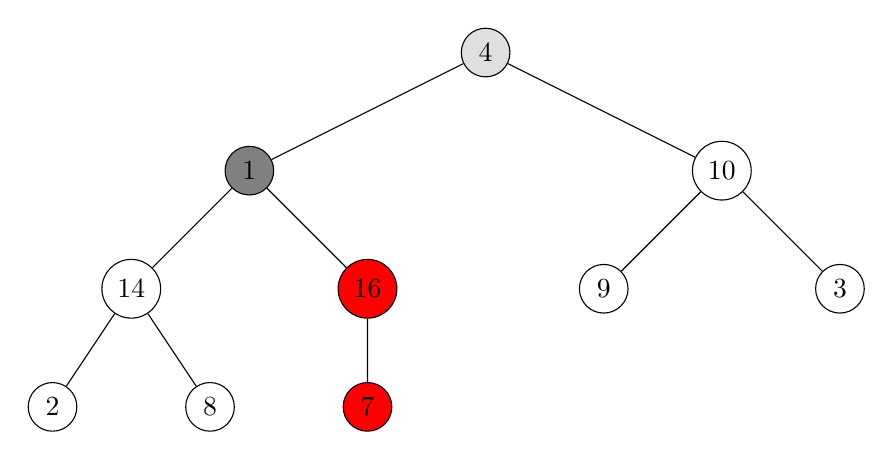
\begin{tikzpicture}[level/.style={sibling distance=60mm/#1}]
\node [circle,draw, fill=gray!25] (z){4}
	child {node [circle, draw, fill=gray] (a) {1}
		child {node [circle, draw] (c) {14}
			child {node [circle, draw] (g) {2}}
			child {node [circle, draw] (h) {8}}
		}
		child {node [circle, draw, fill=red] (d) {16}
			child {node [circle, draw, fill=red] (i) {7}}
		}
	}
	child {node [circle, draw] (b) {10}
		child {node [circle, draw] (e) {9}}
		child {node [circle, draw] (f) {3}}
	}
;
\end{tikzpicture}
\end{center}
Als laatste laten we ook de wortel zakken tot zijn correcte plaats.
\begin{center}
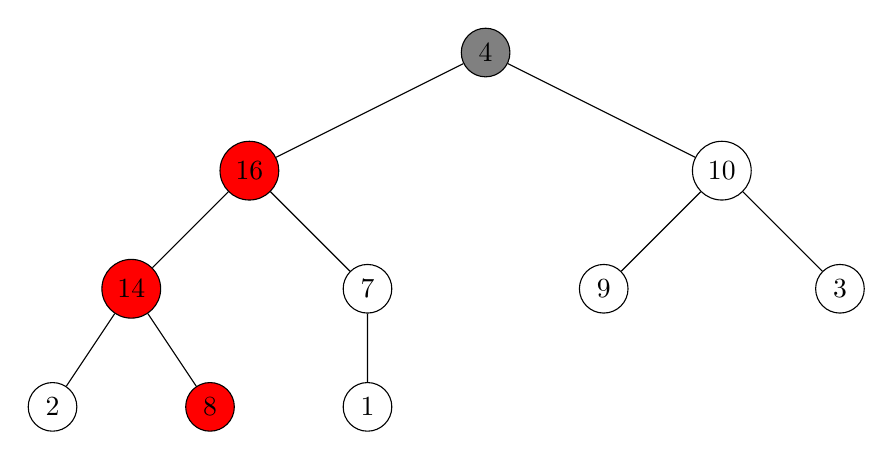
\begin{tikzpicture}[level/.style={sibling distance=60mm/#1}]
\node [circle,draw, fill=gray] (z){4}
	child {node [circle, draw, fill=red] (a) {16}
		child {node [circle, draw, fill=red] (c) {14}
			child {node [circle, draw] (g) {2}}
			child {node [circle, draw, fill=red] (h) {8}}
		}
		child {node [circle, draw] (d) {7}
			child {node [circle, draw] (i) {1}}
		}
	}
	child {node [circle, draw] (b) {10}
		child {node [circle, draw] (e) {9}}
		child {node [circle, draw] (f) {3}}
	}
;
\end{tikzpicture}
\end{center}
De heap wordt uiteindelijk:
\begin{center}
\begin{tikzpicture}[level/.style={sibling distance=60mm/#1}]
\node [circle,draw] (z){16}
	child {node [circle, draw] (a) {14}
		child {node [circle, draw,] (c) {8}
			child {node [circle, draw] (g) {2}}
			child {node [circle, draw] (h) {4}}
		}
		child {node [circle, draw] (d) {7}
			child {node [circle, draw] (i) {1}}
		}
	}
	child {node [circle, draw] (b) {10}
		child {node [circle, draw] (e) {9}}
		child {node [circle, draw] (f) {3}}
	}
;
\end{tikzpicture}
\end{center}
De tabel ziet er nu als volgt uit:
\begin{center}
\begin{tabular}{ |c|c|c|c|c|c|c|c|c|c| }
\hline
16 & 14 & 10 & 8 & 7 & 9 & 3 & 2 & 4 & 1 \\
\hline
\end{tabular}
\end{center}
Nu kan de gerangschikte tabel efficiënt geconstrueerd worden door steeds de wortel van de heap met het laatste blad te wisselen, de heap te verkleinen en dan de \textit{heapvoorwaarde} te herstellen. De knoop met waarde 1 zal zakken via de in het rood aangeduide weg.
\begin{center}
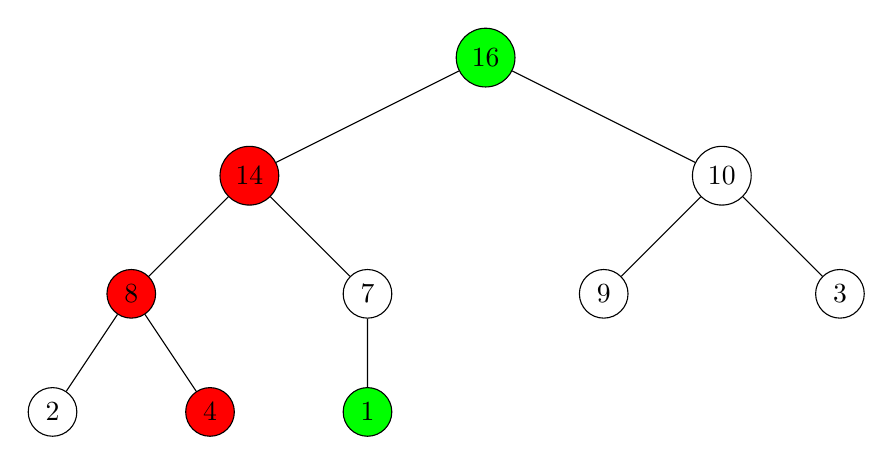
\begin{tikzpicture}[level/.style={sibling distance=60mm/#1}]
\node [circle,draw, fill=green] (z){16}
	child {node [circle, draw, fill=red] (a) {14}
		child {node [circle, draw, fill=red] (c) {8}
			child {node [circle, draw] (g) {2}}
			child {node [circle, draw, fill=red] (h) {4}}
		}
		child {node [circle, draw] (d) {7}
			child {node [circle, draw, fill=green] (i) {1}}
		}
	}
	child {node [circle, draw] (b) {10}
		child {node [circle, draw] (e) {9}}
		child {node [circle, draw] (f) {3}}
	}
;
\end{tikzpicture}
\end{center}
Dit proces gaat verder tot de gerangschikte tabel volledig geconstrueerd is.
\begin{center}
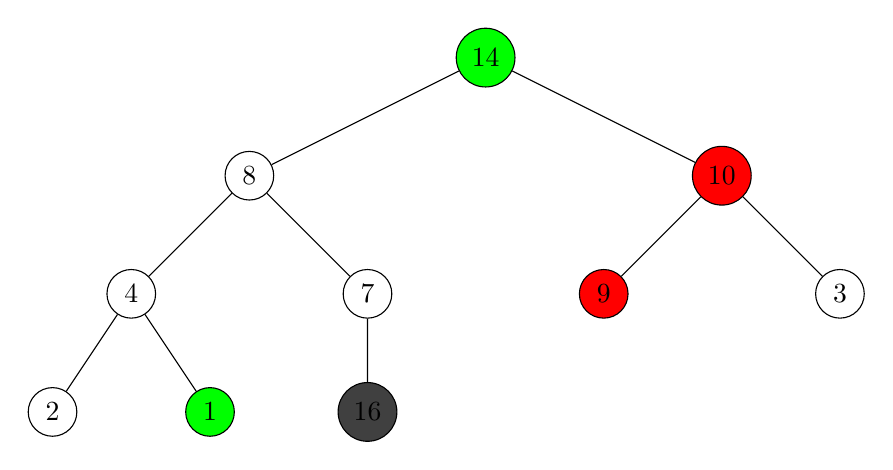
\begin{tikzpicture}[level/.style={sibling distance=60mm/#1}]
\node [circle,draw, fill=green] (z){14}
	child {node [circle, draw] (a) {8}
		child {node [circle, draw] (c) {4}
			child {node [circle, draw] (g) {2}}
			child {node [circle, draw, fill=green] (h) {1}}
		}
		child {node [circle, draw] (d) {7}
			child {node [circle, draw, fill=darkgray] (i) {16}}
		}
	}
	child {node [circle, draw, fill=red] (b) {10}
		child {node [circle, draw, fill=red] (e) {9}}
		child {node [circle, draw] (f) {3}}
	}
;
\end{tikzpicture}

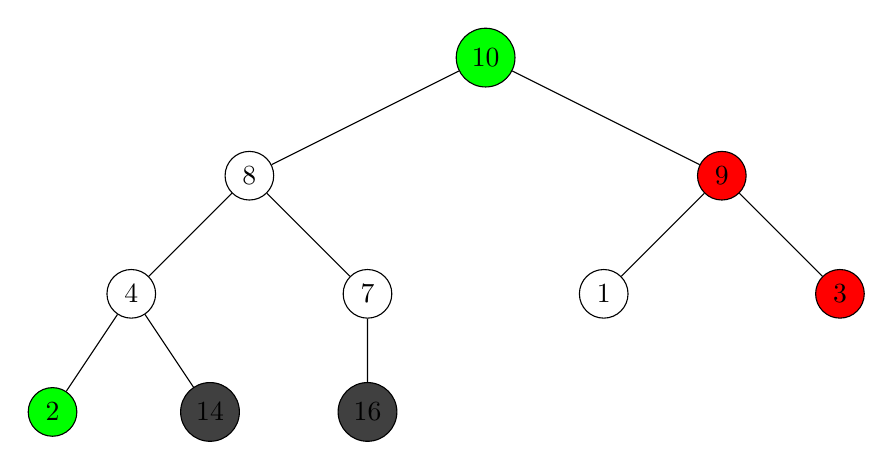
\begin{tikzpicture}[level/.style={sibling distance=60mm/#1}]
\node [circle,draw, fill=green] (z){10}
	child {node [circle, draw] (a) {8}
		child {node [circle, draw] (c) {4}
			child {node [circle, draw, fill=green] (g) {2}}
			child {node [circle, draw, fill=darkgray] (h) {14}}
		}
		child {node [circle, draw] (d) {7}
			child {node [circle, draw, fill=darkgray] (i) {16}}
		}
	}
	child {node [circle, draw, fill=red] (b) {9}
		child {node [circle, draw] (e) {1}}
		child {node [circle, draw, fill=red] (f) {3}}
	}
;
\end{tikzpicture}

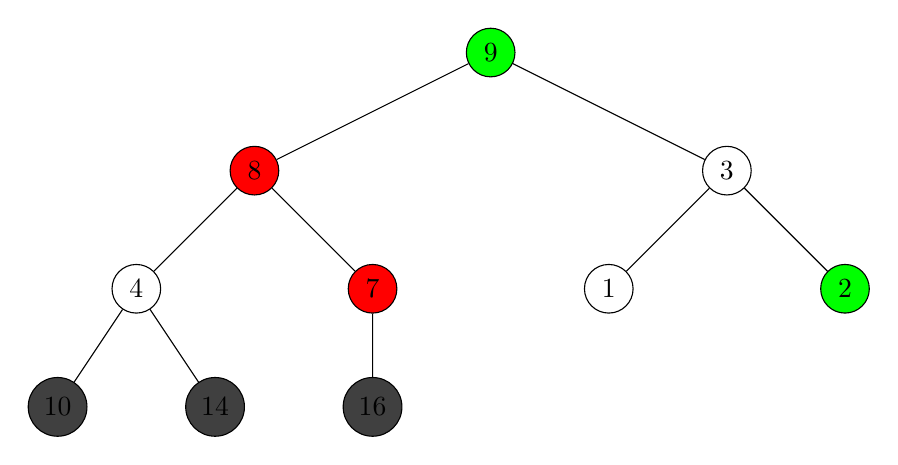
\begin{tikzpicture}[level/.style={sibling distance=60mm/#1}]
\node [circle,draw, fill=green] (z){9}
	child {node [circle, draw, fill=red] (a) {8}
		child {node [circle, draw] (c) {4}
			child {node [circle, draw, fill=darkgray] (g) {10}}
			child {node [circle, draw, fill=darkgray] (h) {14}}
		}
		child {node [circle, draw, fill=red] (d) {7}
			child {node [circle, draw, fill=darkgray] (i) {16}}
		}
	}
	child {node [circle, draw] (b) {3}
		child {node [circle, draw] (e) {1}}
		child {node [circle, draw, fill=green] (f) {2}}
	}
;
\end{tikzpicture}
\end{center}
Ik ga hier geen 25 pagina's vol van die stomme bomen zetten. \textit{Hope you get it by now}.
% subsection voorbeeld (end)

\subsubsection{Complexiteit} % (fold)
\label{sub:heap_sort_heap_sort_complexiteit}
Rangschikken verwijdert $n-1$ keer het wortelelement van de heap. De reconstructie van de heap is iedere keer $O(\lg n)$. Dit maakt heap sort $O(n\lg n)$.
Gemiddelde geval is ook $\Theta(n\lg n)$ (zonder bewijs), testen tonen aan dat dit gedrag zeer consistent is: gemiddelde geval nauwelijks sneller dan slechtste.
% subsection complexiteit (end)

\subsubsection{Waarom Beter?} % (fold)
\label{sub:heap_sort_waarom_beter}
Voor grote $n$ is heap sort sneller dan eenvoudige methodes.
% subsection waarom_beter_ (end)
% subsection heap_sort (end)

\subsection{Merge Sort} % (fold)
\label{sub:merge_sort}
\subsubsection{Doel} % (fold)
\label{sub:merge_sort_doel}
Sorteren van elementen
% subsection doel (end)

\subsubsection{Basisprincipes} % (fold)
\label{sub:merge_sort_merge_sort_basisprincipes}
Merge sort gebruikt de `verdeel en heers' techniek om een rangschik probleem op te lossen. Ze verdeelt het probleem in een aantal \textit{onafhankelijke} deelproblemen. Merge sort zal de tabel iedere keer in twee delen en de deeltabellen sorteren. Dit blijft zo doorgaan tot een tabel met grootte één, deze is namelijk al gesorteerd. Om twee tabellen samen te voegen wordt iedere keer de kleinste elementen van de tabellen te vergelijken en het minimum weg te nemen. Als het einde van één van de deeltabellen bereikt wordt kan de rest van de andere zo overgenomen worden. Merge sort sorteert dus niet ter plaatse, er is een hulptabel nodig met als grootte de grootte van de kleinste deeltabel. Merge sort is wel stabiel zolang bij gelijke kleinste waarden altijd de linkse waarde genomen wordt als minimum.

Er bestaat ook een niet recursieve versie. Deze gebruikt een \textit{bottom-up} verwerking. De tabel van begin tot einde overlopen, waarbij alle paren opeenvolgende elementen samengevoegd worden tot deeltabellen van lengte twee. Dan opnieuw en samenvoegen tot lengte vier, enz.
% subsection basisprincipes (end)

\subsubsection{Voorbeeld} % (fold)
\label{sub:merge_sort_voorbeeld}
Verdelen van tabel in deeltabellen:
\begin{figure}[h]
	\centering
	\includegraphics[width=0.5\textwidth]{merge_sort_divide}
	\caption{Verdelen tabel in deeltabellen}
	\label{fig:merge_sort_divide}
\end{figure}

Samenvoegen deeltabellen:
\begin{figure}[h]
	\centering
	\includegraphics[width=0.5\textwidth]{merge_sort_merge}
	\caption{Samenvoegen deeltabellen}
	\label{fig:merge_sort_merge}
\end{figure}
% subsection voorbeeld (end)

\subsubsection{Complexiteit} % (fold)
\label{sub:merge_sort_complexiteit}
\textit{Best-}, \textit{Worst-} en \textit{Average-case} zijn allemaal hetzelfde. Merge sort is dus $\Theta(n\lg n)$

% subsection complexiteit (end)

\subsubsection{Waarom Beter?} % (fold)
\label{sub:merge_sort_waarom_beter}
Mergesort is asymptotisch even efficiënt als \hyperref[sub:heap_sort]{heap sort}, maar blijkt iets sneller te zijn met een goede implementatie. Oorspronkelijke volgorde van de elementen speelt nauwelijks een rol voor deze methode, wat haar gedrag dus heel consequent maakt: \textit{Best-}, \textit{Worst-} en \textit{Average-case} zijn allemaal hetzelfde.
% subsection waarom_beter_ (end)

\subsubsection{Mogelijke Optimalisaties} % (fold)
\label{sub:merge_sort_mogelijke_optimalisaties}
\begin{itemize}
	\item \hyperref[sub:insertion_sort]{Insertion Sort} gebruiken als de deeltabellen klein genoeg zijn. Het is efficiënter dan de volledige recursie opnieuw te doen voor kleine tabellen. Insertion sort zorgt er ook niet voor de het algoritme niet meer stabiel is.
	\item Als er een hulptabel van grote $n$ is, kan er afwisselend samengevoegd worden. Waardoor nutteloos kopiëren voor iedere \textit{merge} niet meer nodig is.
\end{itemize}

% subsection mogelijke_optimalisaties (end)

\subsubsection{Analyse/Bewijs complexiteit} % (fold)
\label{sub:merge_sort_analyse_bewijs_complexiteit}
\begin{itemize}
	\item \textit{Recursieve versie}: 
\end{itemize}

% subsection analyse_bewijs_complexiteit (end)
% subsection merge_sort (end)



\subsection{Skelet} % (fold)
\label{sub:skelet}
\subsubsection{Doel} % (fold)
\label{sub:doel}
Sorteren van elementen
% subsection doel (end)

\subsubsection{Basisprincipes} % (fold)
\label{sub:basisprincipes}

% subsection basisprincipes (end)

\subsubsection{Voorbeeld} % (fold)
\label{sub:voorbeeld}

% subsection voorbeeld (end)

\subsubsection{Complexiteit} % (fold)
\label{sub:complexiteit}

% subsection complexiteit (end)

\subsubsection{Waarom Beter?} % (fold)
\label{sub:waarom_beter}

% subsection waarom_beter_ (end)

\subsubsection{Mogelijke Optimalisaties} % (fold)
\label{sub:mogelijke_optimalisaties}

% subsection mogelijke_optimalisaties (end)

\subsubsection{Analyse/Bewijs complexiteit} % (fold)
\label{sub:analyse_bewijs_complexiteit}

% subsection analyse_bewijs_complexiteit (end)
% subsection skelet (end)

\newpage

\section{Gegevensstructuren I\label{gegI}}
\subsection{Heaps} % (fold)
\label{sub:heaps}
Een heap is een \textit{complete binaire boom}, waarvan de elementen voldoen aan de \textit{heapvoorwaarde}. De \textit{heapvoorwaarde} van een \textit{stijgende} heap (of \textit{maxheap}) zegt dat de sleutel van de ouder minstens even groot moet zijn als deze van zijn kind(eren). De onderlinge volgorder van de sleutels van de kinderen maakt hierbij niet uit. De kinderen van iedere knoop $i$ zijn te vinden op indexen $2i+1$ en $2i+2$. De ouder van een knoop is te vinden op index $\lfloor(i-1)/2\rfloor$. De hoogte van een heap $h = \lfloor \lg n \rfloor$
\subsubsection{Operaties} % (fold)
\label{sub:heaps_operaties}
\begin{itemize}
	\item \textit{Element toevoegen}. Nieuwe knoop maken op laagste niveau (\textbf{bij tabelindex $n + 1$}). Nu moet enkel de heapvoorwaarde nog herstelt worden: Zolang de nieuwe knoop een ouder heeft met een grotere sleutel wisselen deze knopen. Zodat de nieuwe knoop stijgt in de heap tot hij een ouder heeft met een grotere of even grote sleutel. Deze methode kan vergeleken worden met \hyperref[sub:insertion_sort]{insertions sort}: Kleinere elementen worden ook opgeschoven, maar deze keer wel via de weg in de heap tussen wortel en de nieuwe knoop.
	\item \textit{Wortelelement vervangen} door nieuwe knoop $g$. De \textit{heapvoorwaarde} kan verbroken worden als de nieuwe waarde kleiner is. In dit geval wisselen we de knoop met zijn grootste kind. Zo laten we de nieuwe waarde zakken in de heap tot op zijn correcte plaats. 
	\item \textit{Wortelelement verwijderen}. Deze operatie komt neer op het vervangen van de wortel door het laatste element in de kleiner geworden heap.
	\item \textit{Element van een willekeurige knoop vervangen}. De \textit{heapvoorwaarde} kan maar in één richting verstoord worden. Richting de wortel als de nieuwe waarde groter is, dan is het analoog aan een nieuwe waarde toevoegen aan een heap. Als het nieuwe element kleiner is dan is de situatie analoog aan het wortelelement vervangen, maar dan toegepast op de deelheap.
\end{itemize}
% subsection operaties (end)
\subsubsection{Constructie} % (fold)
\label{sub:heaps_constructie}
\begin{itemize}
	\item \textit{Door toevoegen}. Elementen één voor één toevoegen aan een oorsponkelijk ledige heap. Tabel kan ter plaatse getransformeerd worden tot heap.
	\item \textit{Door samenvoegen van deelheaps}. Beschouw tabel direct als \textit{complete, binaire boom} en itereer over de eerste $\lfloor n/2 \rfloor$ elementen van rechts naar links. Als een van deze knopen een kind heeft met een grotere waarde blijven we deze knoop wisselen met zijn grootste kind tot de knoop geen kinderen meer heeft met een grotere waarde of een blad geworden is.
\end{itemize}
\hyperref[sub:heap_sort_voorbeeld]{Voorbeeld van constructie met samenvoegen}.
% subsection constructie (end)

\subsubsection{Sterktes en Zwaktes} % (fold)
\label{sub:heaps_sterktes_en_zwaktes}
\begin{itemize}
	\item Meeste bewerkingen op een heap zijn efficiënt omdat hun tijdsduur begrenst wordt door de hoogte van de heap, die veel kleiner is dan het aantal elementen.
\end{itemize}

% subsection sterktes_en_zwaktes (end)

\subsubsection{Complexiteit van Operaties} % (fold)
\label{sub:heaps_complexiteit_van_operaties}
\begin{itemize}
	\item \textit{Element toevoegen}. Het aantal keer dat we knopen moeten wisselen is beperkt door de hoogte van de heap. Een element toevoegen heeft dus $O(h) = O(\lg n)$ operaties.
	\item \textit{Wortelelement vervangen}. De langste weg langs waar de nieuwe wortel zou moeten zakken is nog steeds $h$ dus de complexiteit blijft $O(h) = O(\lg n)$. Er moeten wel meer vergelijkingen gebeuren (knoop heeft max 2 kinderen en max 1 ouder).
	\item \textit{Wortelelement verwijderen}. Aangezien dit analoog is aan het wortelelement vervangen is deze operatie ook $O(\lg n)$.
	\item \textit{Element van willekeurige knoop vervangen}. Ook hier is de grootste afgelegde weg van een vervangen knoop $h$. De complexiteit van deze operatie is dus ook $O(h) = O(\lg n)$
	\item \textit{Constructie door toevoegen}. Er moet $n-1$ keer een element toegevoegd worden aan de heap (het eerste element staat al goed). In het slechtste geval moet iedere knoop die toegevoegd wordt de volledige hoogte van de heap doorlopen (nieuwe wortel worden). Als dan ook nog eens het laatste niveau volledig opgevuld wordt krijgen we een bovengrens voor performantie. Het aantal keer dat gewisseld wordt per niveau kan uitgedrukt worden ifv de hoogte: $2^hh$. Het totaal aantal wissels voor de volledige heap is dus maximaal $\sum_{i=0}^{h} 2^hh$. Door volgende afschatting te gebruiken kan de complexiteit voor het opstellen van de heap berekend worden:
	$$\sum_{i=0}^{h} 2^hh \leq 2^{h+1}h = 2^{\lg n + 1}\lg n = \lg n(n+1) = O(n\lg n)$$
	\item \textit{Constructie door samenvoegen}. Veel efficiënter dan toevoegen. Heap wordt van onder naar boven opgebouwd. In het slechtste geval moeten alle eerste $\lfloor n/2 \rfloor$ elementen naar bladeren van de boom gebracht worden. Het aantal wissels per niveau is $2^i(h-i)$. Het maximale aantal wissels is dus $\sum_{i=0}^{h-1} 2^i(h-i)$. Ook hier kan een afschatting gebruikt worden om de complexiteit te berekenen:
	$$\sum_{i=0}^{h-1} 2^i(h-i) \leq 2\cdot 2^{h+1} = 2\cdot 2^{\lg n + 1} = 2(n+1) = O(n)$$
\end{itemize}
% subsection complexiteit_van_operaties (end)

\subsubsection{Toepassingen} % (fold)
\label{sub:heaps_toepassingen}
\hyperref[sub:heap_sort]{Heap Sort}
% subsection toepassingen (end)
% subsection heaps (end)



\subsection{GegSkelet} % (fold)
\label{sub:gegskelet}
\subsubsection{Operaties} % (fold)
\label{sub:operaties}

% subsection operaties (end)

\subsubsection{Sterktes en Zwaktes} % (fold)
\label{sub:sterktes_en_zwaktes}

% subsection sterktes_en_zwaktes (end)

\subsubsection{Complexiteit van Operaties} % (fold)
\label{sub:complexiteit_van_operaties}

% subsection complexiteit_van_operaties (end)

\subsubsection{Analyse/Bewijs Complexiteit van Operaties} % (fold)
\label{sub:analyse_bewijs_complexiteit_van_operaties}

% subsection analyse_bewijs_complexiteit_van_operaties (end)

\subsubsection{Toepassingen} % (fold)
\label{sub:toepassingen}

% subsection toepassingen (end)
% subsection gegskelet (end)
\newpage

\section{Graafalgoritmen I\label{graafI}}

\end{document}